% prima bisogna dichiarare la \documentclass[opzioni]{classe} di che tipo è?
%\begin{document} inizia il corpo
% qui c'è il test vero e proprio dove tratta di cosa stiamo paralndo
%\end{document}
%----------------------%
% \usepackage{pacchetto} per usare un pacchetto
% \author{} dice chi è l'autore
% \date{} vuota non dice niente, mentre, di default è la data di compilazione
% \maketitle produce l'intestazione
% \tableofcontents produce l'indice dei capitoli
% \section{titolo sezione} produce una sezione
% --------------------%
% \usepakage[utf8]{inputenc} per le lettere della tastiera
% \usepakage{indentfirst} per indentare automaticamente

\documentclass{article}

\title{Tutorial \LaTeX}
\author{Petru Rusu}
\date{}

\usepackage{afterpage}
\usepackage{tikz}
\usetikzlibrary{positioning}
\usepackage[utf8]{inputenc}
\usepackage{lipsum}
\usepackage{indentfirst, lstautogobble} 
\usepackage{listings}
\usepackage{xcolor}
\usepackage{tikz}
\usepackage{array}
\usepackage{tikz}

% Definizione dello stile per il codice
\lstset{
    language=C,
    basicstyle=\small\ttfamily,
    keywordstyle=\color{blue},
    commentstyle=\color{green!60!black},
    stringstyle=\color{red},
    showstringspaces=false,
    breaklines=true,
    captionpos=b,
    numbers=left,
    numberstyle=\tiny,
    numbersep=5pt,
    xleftmargin=3mm,
    showstringspaces=false,
    breaklines=true,
    frameround=ffff,
    rulecolor=\color{black},
    autogobble=true,
}

\setlength{\parindent}{0pt}

\begin{document}
    \maketitle
    \tableofcontents
    \newpage 

    \section{The starting}
        \subsection{Low level vs high Level}
        when you write a programs in any language, this program have to be converted in machine language, after the CPU will execute the task.
        There are two type of language: low level and high level.
        
        \begin{itemize}
            \item \textbf{Low level:} is really close to the hardware and we    should have a good knowledge about CPU.
               \\
                For example we have to know that when we sum 1 + 1 we create a space in RAM that occupies 20 bits, where 4 is for declare the +, 1 byte is for memorize 1 and the other byte is for memorize the last 1, it is the arrays.
                They usually use a compiler
                \begin{center}
                    \begin{tabular}{|*{10}{c|}}
                        \hline
                        1 & 2 & 3 & 4 & 5 & 6 & 7 & 8 & 9 & 10 \\
                        \hline
                        11 & 12 & 13 & 14 & 15 & 16 & 17 & 18 & 19 & 20 \\
                        \hline
                    \end{tabular}
                \end{center}
            \item \textbf{High level:} allow developers to write more abstract and readable code, away from specific machine or hardware details. This fosters better code understanding and facilitates software maintenance and updates. but usually they are slower than low level code.
            They usually use a interpreter
            
        \end{itemize}
        \subsubsection{compiler vs interpreter}
            \begin{itemize}
                \item \textbf{Compiler:} C code$\rightarrow $ Compiler$ \rightarrow$ machine code. 
                \\ The code first is translated, and after is executed.
                \\But it means that is most difficult to correct errors because will show us all errors after the compiling. we do not need about the source code. the compiler do not stay in memory when we execute the code.

                \item \textbf{Interpreter: } code$\rightarrow $ interpreter$ \rightarrow$ out put 
                \\The while the code is translated the machine execute, so the machine execute line per line. Do not produce object code.
                \\It means that is most easier to correct errors because when it encounters an error it will stop compilation and show it to us one line at a time. and we need about the source code. Interpreter have to stay in memory because is he that execute the code.
                
            \end{itemize}
        
     
    \subsection{What is Compilation?}
         Is the process of converting the source code into object code. It is done with the help of the compiler. The compiler checks for errors.
        %----------------%
        \newpage
            \subsubsection{How Does It Work?}
                \begin{itemize}
                    \item Processor: Removes the comments and expands the library with the code. \texttt{hello.c} $\rightarrow$ \texttt{hello.i} (expanded code), it means that replaces all the line that start with \# with the value, and remove \#
                    %----------------%
                    \item Compiler: Converts this code into assembly code pre-processed code, and check for syntax errors\\
                    assembly code \texttt{hello.i} $\rightarrow$ \texttt{hello.s} (assembly code)
                    %----------------%
                    \item Assembler: Converts the assembly code into machine code by using an assembler. \texttt{hello.s} $\rightarrow$ \texttt{hello.o}
                    %----------------%
                    \item Linker: Its main work is to combine the object code of the library file with the object code of our program. It links the object code of these files to our program.
                \end{itemize}
                
    \section{variables in c}
        A variable is a name for the memory location, is used for store data.
        \subsection{constants}
            \#define pi 3.14 is a symbolic constant, is used for define a fix constant.\\ In C we have 2 type of constants:
            \begin{itemize}
                \item the first is the numeric:
                \begin{itemize}
                    \item integer numbers, that can be represented in different bases:
                    \begin{itemize}
                        \item decimal $\rightarrow$  base10 = 0-9, by default
                        \item octal $\rightarrow$  base8 = 0-7, add a 0 before (05)
                        \item hexadecimal $\rightarrow$  base16 = 0-15, add 0x before (0xf)
                    \end{itemize}
                    \item float numbers [ decimal part, decimal point, fractional part ].
                        \begin{itemize}
                            \item 12.54
                        \end{itemize}
                \end{itemize}
                \item the second is the
                
                
                characters
                    \begin{itemize}
                        \item the first is the single character constant
                            \begin{itemize}
                                \item are like 'a', 'b', '2'
                                \item 5 $\neq$ '5'
                                \item we can represent a number like a char following the ASCII rule 
                                \begin{lstlisting}
                                    printf("%d", 'a');//represent a char in number 
                                    printf("%c", 97);//represent a number in a char 
                                \end{lstlisting}
                            \end{itemize}
                            \item string constants:
                                \begin{itemize}
                                    \item are written inside double quotes: "i am a string"
                                    \item 'a' $\neq$ "a"
                                    \item at the finish of every string put a \textbackslash 0
                                \end{itemize}
                    \end{itemize}
            \end{itemize}

        \subsection{how to create them}
         The syntax for declare the variable is: \texttt{type variable-list}; after that we have to initialize a variable saying what data it have to contain: \texttt{variable = 10;}
         
        \begin{lstlisting}
            int main()
            {
                int a;  // declaration
                a = 10; // initialization

                // we can also do this
                int a = 100, b = 200;

                const int c = 10; 
                c = 12; // it is a error, we cannot change a constant
            }
        \end{lstlisting}

        \subsection{rules for defining variables}
            \begin{itemize}
                \item A variable can have alphabets, digits, and underscore.
                \item A variable name can start with the alphabet, and underscore only. It can't start with a digit.
                \item No whites-pace is allowed within the variable name.
                \item A variable name must not be any reserved word or keyword, e.g. int, float, etc.
            \end{itemize}
            
        \subsection{Data Type in C}
            the c language is a typed language; it means that you have to write what type and what size of data the variable have to contain. datatype are divided in:
            \begin{center}
                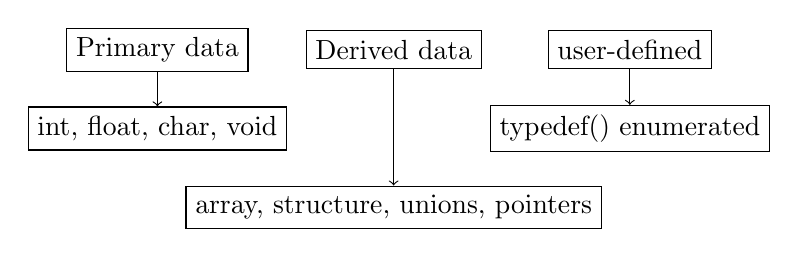
\begin{tikzpicture}
                    % Nodes
                    \node (concept1) [draw, rectangle] {Primary data};
                    \node (concept1-1) [draw, rectangle, below of=concept1] {int, float, char, void};
                    %------------------------------------------------------------------------------%
                    \node (concept2) [draw, rectangle, right of=concept1, xshift=2cm] {Derived data};
                    \node (concept2-1) [draw, rectangle, below of=concept2, yshift=-1cm] {array, structure, unions, pointers};
                    %------------------------------------------------------------------------------%
                    \node (concept3) [draw, rectangle, right of=concept2, xshift=2cm] {user-defined};
                    \node (concept3-1) [draw, rectangle, below of=concept3] {typedef() enumerated};
                    % Arrows
                    \draw[->] (concept1) -- (concept1-1);
                    \draw[->] (concept2) -- (concept2-1);
                    \draw[->] (concept3) -- (concept3-1);
                    
                \end{tikzpicture}
            \end{center}

            \subsubsection{Primary data:}
            the value of this data type can change, it depend if u are using a 32 bit machine, a 16 bit machine, a 64 bit machine
            \renewcommand{\arraystretch}{1.5} % Imposta lo spazio verticale
            \begin{center}
                \begin{tabular}{| l | l | c | c |}
                    \hline
                    \textbf{Name of data} & \textbf{Range of number} & \textbf{bytes} & \textbf{Symbol} \\
                    \hline
                    \hline
                    char & -128 to 127 & 1 & \%c \\
                    unsigned char & 0 to 255 & 1 & \%c \\
                    signed char & -128 to 127 & 1 & \%d \\
                    \hline
                    short int & -32768 to 32767 & 2 & \%h \\
                    unsigned short int & 0 to 65535 & 2 & \%h \\
                    int & -2147483648 to 2147483647 & 4 & \%d \\
                    unsigned int & 0 to 4294967295 & 4 & \%u \\
                    long int & -2147483648 to 2147483647 & 4 & \%ld \\
                    unsigned long int & 0 to 4294967295 & 4 & \%lu \\
                    long long int & -9.223 $\times 10^{18}$ to 9.223 $\times 10^{18}$ & 8 & \%lld \\
                    unsigned long long int & 0 to 18446744073709551615 & 8 & \%llu \\
                    \hline
                    float & 6-9 digits & 4 & \%f \\
                    double & 15-17 digits & 8 & \%lf \\
                    long double & 18-19 digits & 16 & \%Lf \\
                    \hline
                    void & represents absence & 0 & --- \\
                    \hline
                \end{tabular}
            \end{center}

            \subsubsection{What happens if we take a value that is over the range?}
                For example take the short int data type and say that: \texttt{short x = 32768}, it will not get us a error, but will get us the position of the next value, like a wheel \\ \\
                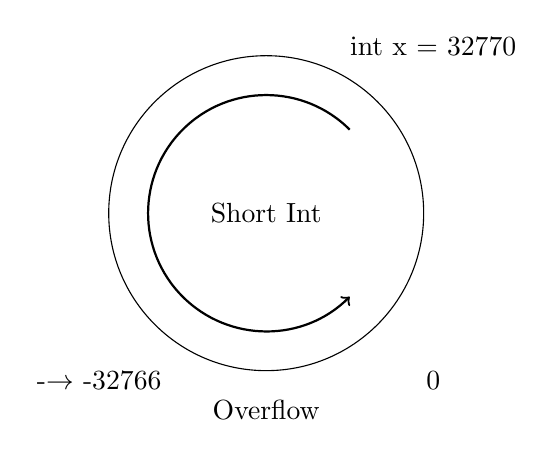
\begin{tikzpicture}
                    % Disegna un cerchio come rappresentazione visiva della ruota
                    \draw (0,0) circle (2cm);
                    % Disegna una freccia per rappresentare il "sorpasso" dell'overflow
                    \draw[->,thick] (45:1.5cm) arc (45:315:1.5cm);
                    % Etichette
                    \node at (0,0) {Short Int}; % Etichetta per il tipo di dato
                    \node at (0,-2.5) {Overflow}; % Etichetta per l'overflow
                    % Aggiunge numeri accanto alla ruota
                    \foreach \angle/\label in {45/ int x = 32770, -45/0, -135/ -$\rightarrow$ -32766}
                    \node at (\angle:3cm) {\label};
                \end{tikzpicture}

        \section{}
            
        
        
\end{document}



